\section{Theoretical Foundations}
This section gives a theoretical overview of FEM and the MFEM library, using mathematical formulations and figures.
\subsection{Finite Element Framework}
To apply MFEM to specific problems, various classes and functions are utilized. An example is the Poisson problem with homogeneous boundary conditions, which involves finding a function u : $\Omega$ → R that satisfies:
-$\Delta$u = f in $\Omega$.
The solution is approached through FEM, leading to the integral form shown in equation \ref{eq}:
\begin{equation}
    \int_{\Omega} \nabla u_h \nabla v_h = \int_{\Omega} f v_h.
    \label{eq}
\end{equation}
By defining a basis function $\phi$ for space $V_h$, this integral is reformulated and solved using appropriate methods.

\subsection{Types of Meshes}
MFEM supports various mesh types like triangular and hexahedral. Meshes in MFEM have two aspects: topological data (e.g., connectivity) and geometric data (e.g., vertices' coordinates). Mesh element shapes are defined through mapping, as shown in Figure \ref{figure_1}, with the equation:

\begin{figure}[hbt!]
    \centering
    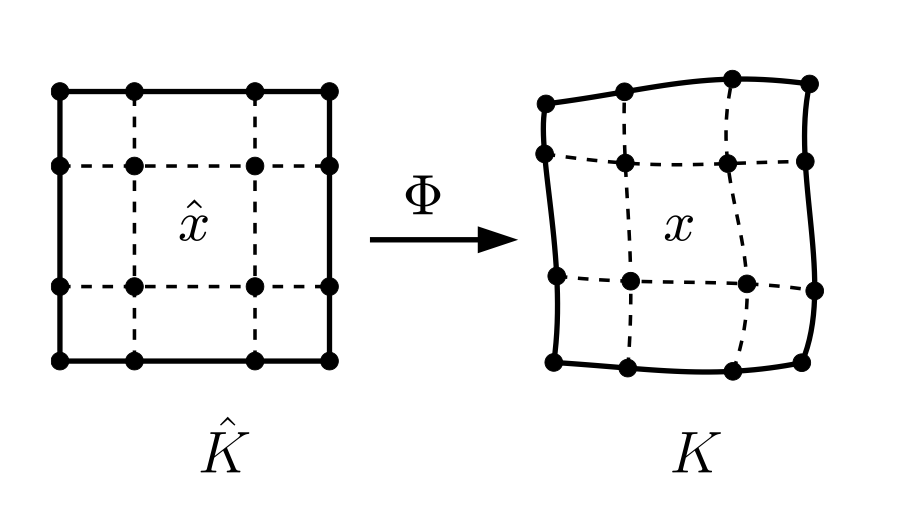
\includegraphics[width=0.5\textwidth]{figures/f1.png}
    \caption{The mapping of an elements}
    \label{figure_1}
\end{figure}

\begin{equation}
    \Omega(x) = \sum_{i=1}^N x_{K_i} w(x).
\end{equation}

MFEM also handles non-conforming, NURBS, and parallel meshes.
